\chapter{Budowa bazy}
\label{sec:robot}
\section{Dookólna platforma mobilna}
	\begin{figure}[H]
	\centering
	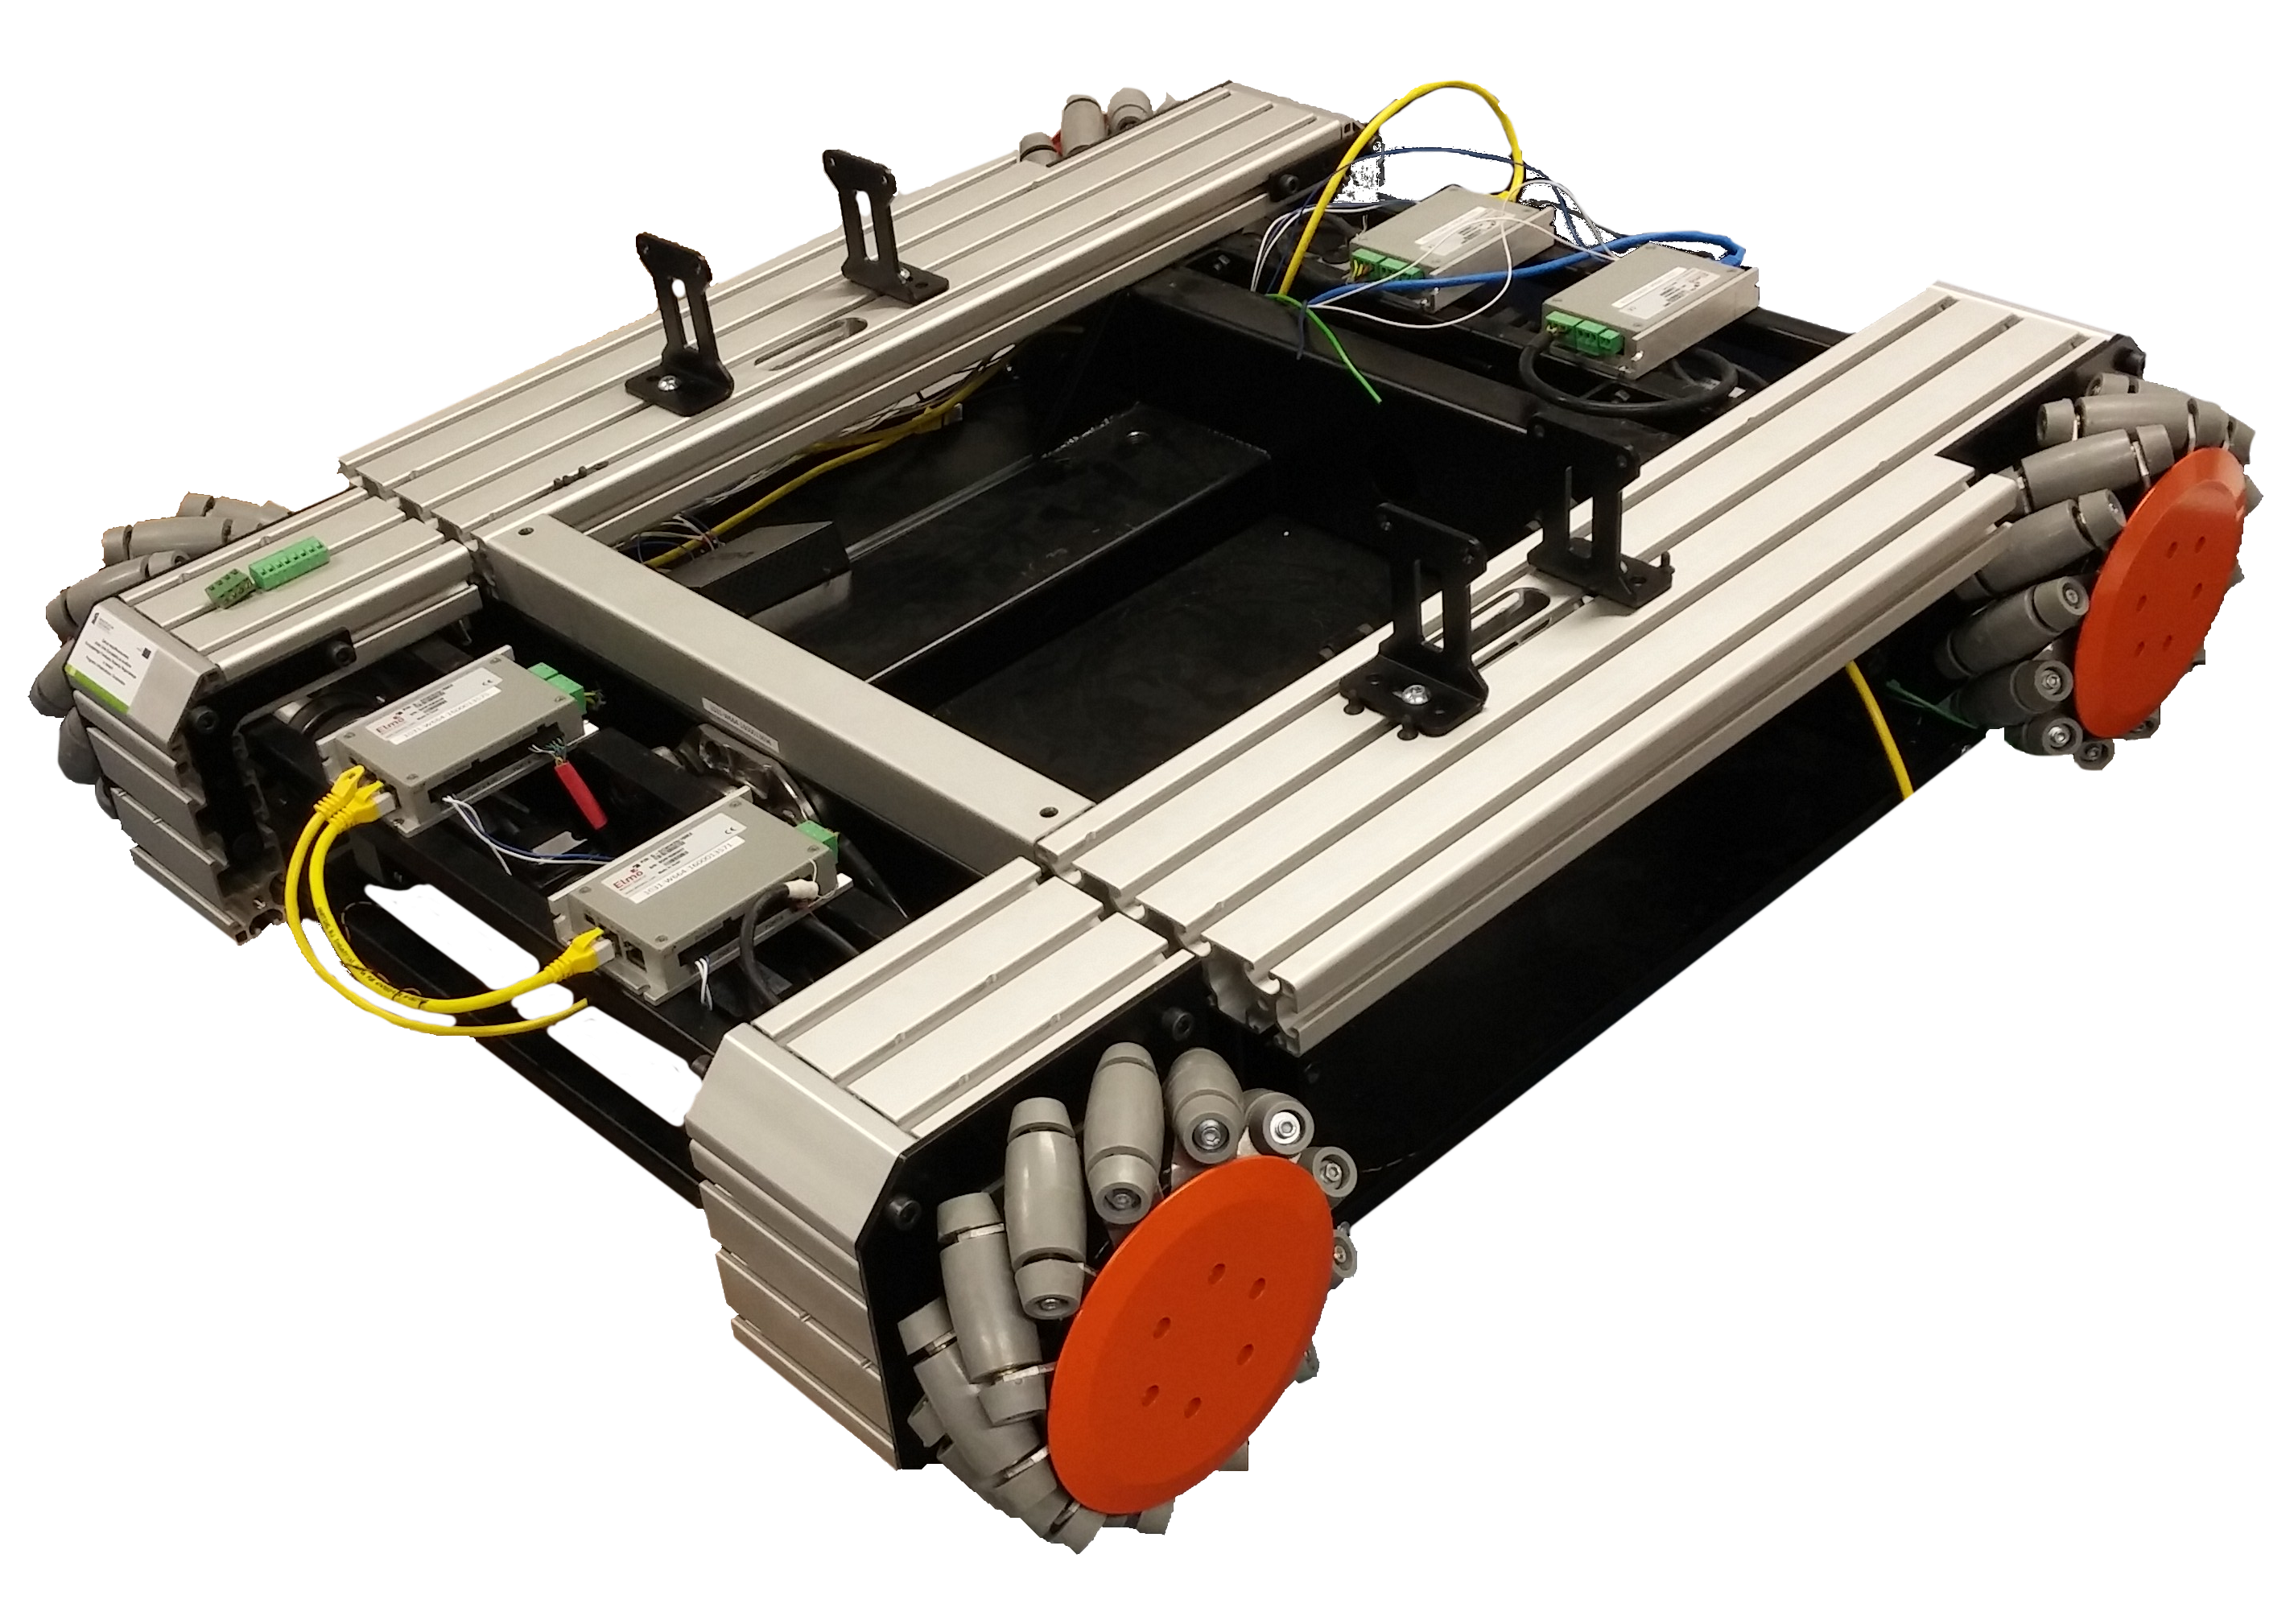
\includegraphics[width=0.8\textwidth]{graphics/base_photo.png}
	\caption{Dookólna baza mobilna na kołach szwedzkich.}
	\label{fig:base_photo}
	\end{figure} 

	Jest to duża, prostokątna baza dookólna, poruszająca się na czterech kołach szwedzkich, rysunek \ref{fig:base_photo}.
	Koła są stałe, parami przytwierdzone do dwóch osi.
	Każde koło jest napędzane osobno przez podłączony bezpośrednio serwomotor, 
	zatem może mieć prędkość i kierunek obrotu niezależny od pozostałych kół, kierunku poruszania się robota, oraz jego orientacji.
	Każdy z serwomotorów ma także wbudowany enkoder.
	Sterownik enkodera nadaje za pomocą sieci aktualny kąt i prędkość obrotu.

	Jest to jeden z najpopularniejszych typów dookólnych platform mobilnych, mających zastosowanie także w innych robotach, jak na przykład Kuka Youbot, rysunek \ref{fig:kuka_youbot}.
	Należy zwrócić uwagę na charakterystyczne ustawienie kół, identyczne jak w opisywanej platformie na rysunku \ref{fig:base_photo}.
	
	Istnieją także roboty z trzema kołami szwedzkimi, w których koła rozstawione są na wierzchołkach trójkąta równobocznego.
	Pomimo prostszej budowy i takiej samej liczby stopni swobody, jak czterokołowa wersja, stabilność takiej konstrukcji jest gorsza \cite{extra_axis}.
	Ponieważ jest to robot transportowy, to stabilność odgrywa tu ważną rolę i czterokołowa konstrukcja jest wskazana.

	\begin{figure}[H]
	\centering
	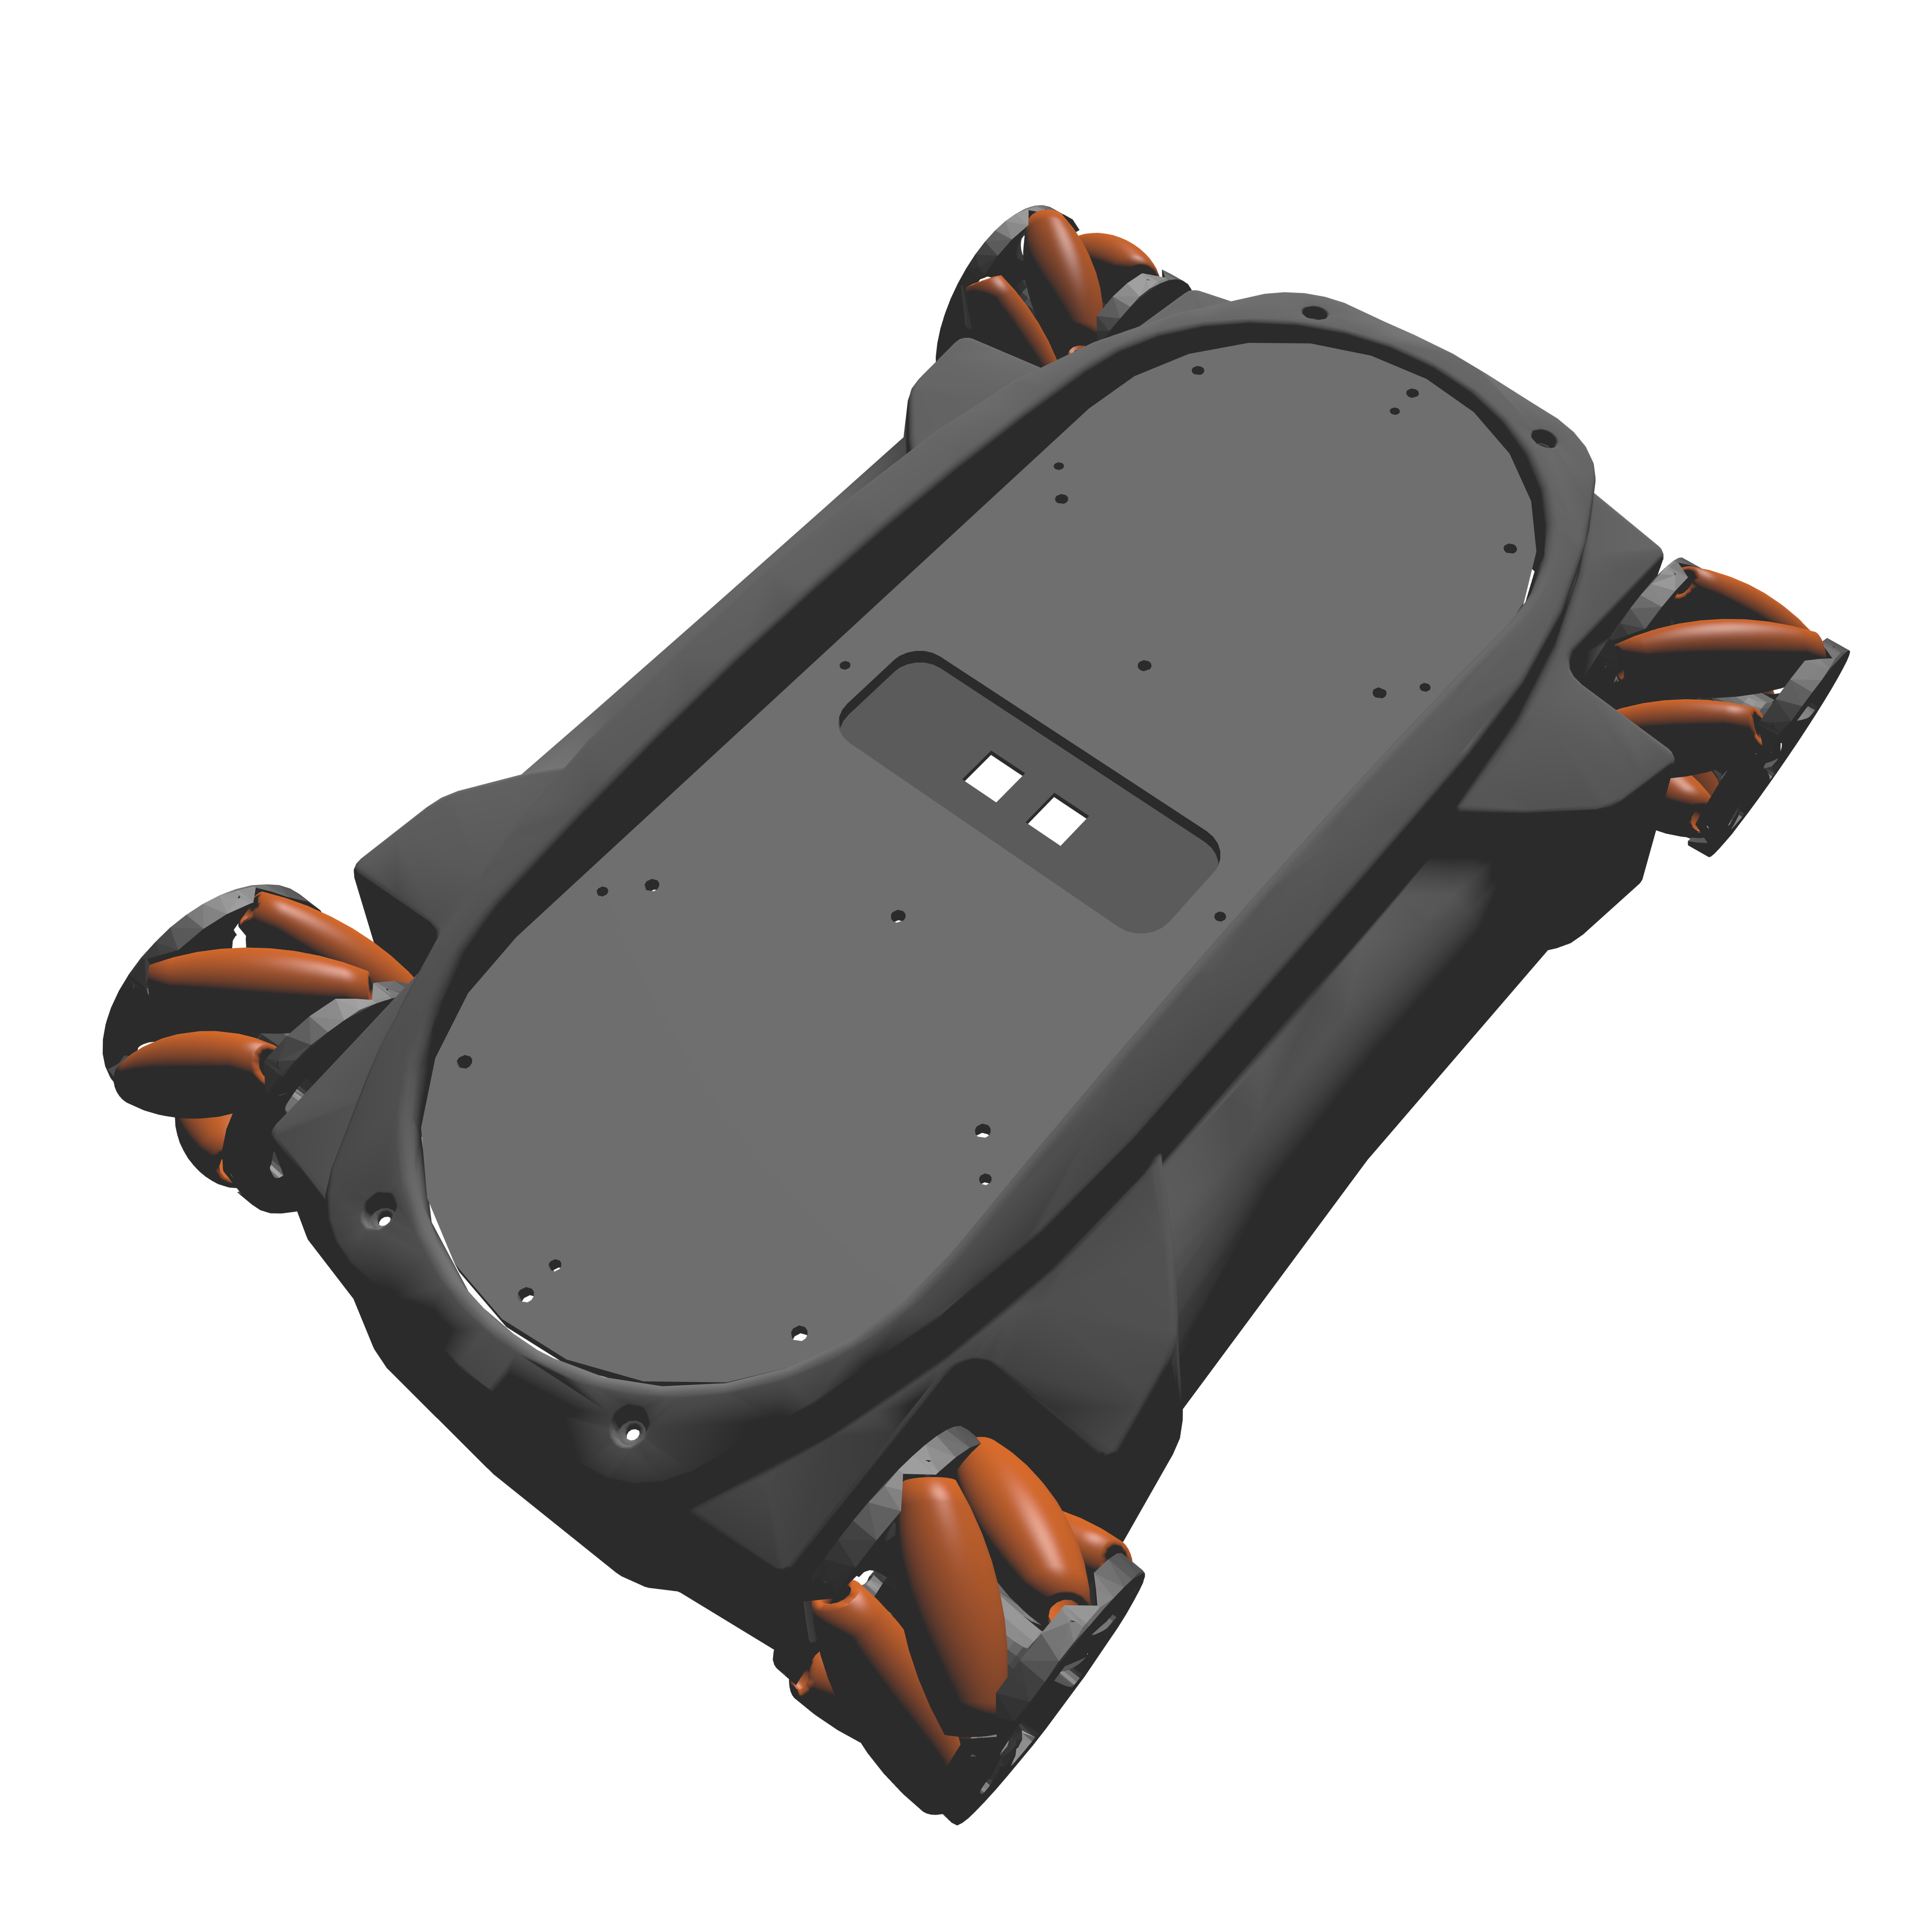
\includegraphics[width=0.5\textwidth]{graphics/kuka_youbot.png}
	\caption{Platforma wycofanego już ze sprzedaży robota Kuka Youbot.}
	\label{fig:kuka_youbot}
	\end{figure} 

	Odpowiedni obrót kół względem bazy, pozwala na jej ruch w dowolnym kierunku, niezależnym od orientacji robota, patrz rysunek \ref{fig:mecanum_dirs}.
	Jest możliwe także obracanie bazą, gdy ta porusza się w dowolnym kierunku, bądź stoi w miejscu.
	
	\begin{figure}[H]
	\centering
	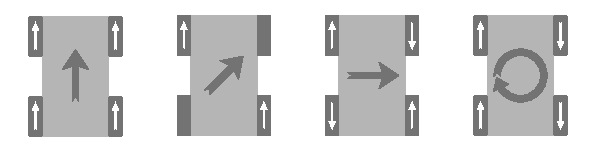
\includegraphics[width=0.8\textwidth]{graphics/mecanum_dirs.pdf}
	\caption{Podstawowe kierunki ruchu robota o napędzie wielokierunkowym.}
	\label{fig:mecanum_dirs}
	\end{figure} 
	
	Przykładowo, poruszając tylko przeciwległymi kołami po przekątnej, robot będzie mógł poruszać się po skosie, bez zmiany orientacji bazy.
	A jeśli do tego dodać obrót kół drugiej przekątnej, w odwrotnym kierunku, wtedy pojazd zacznie się poruszać w bok, pomimo faktu, że koła nie są skrętne i 
	nie mogą ustawić się zgodnie z kierunkiem jazdy.
	Trasa, po której porusza się robot, przy stałej prędkości kół, zawsze jest łukiem okręgu. W szczególnym przypadku można uznać prostą za okrąg o nieskończonym promieniu, a punkt za okręg o zerowym. 
	Wynika to z faktu, że każdy obiekt, który ma jednostajną prędkość i stały kierunek w lokalnym układzie współrzędnych oraz stałą prędkość kątową, będzie się poruszał po łuku.
	Zależność tego promienia okręgu $R$ od prędkości liniowej $v$ i prędkości kątowej $\omega$, wyraża się wzorem $R = \frac{v}{\omega}$.

	Baza mobilna będzie podstawą robota manipulującego Velma, tworząc razem manipulator mobilny.
	Velma to dwuramienny robot, wyposażony w dwa chwytaki o wielu przegubach, patrz rysunek \ref{fig:velma}.
	Taka budowa wymaga szerokiej podstawy, aby zachować bezpieczną równowagę całości.
	Jeżdżąc na tej bazie, robot może się przemieszczać i obracać w dowolnym kierunku, aby uzyskać lepszy dostęp do manipulowanych obiektów.

	\begin{figure}[H]
	\centering
	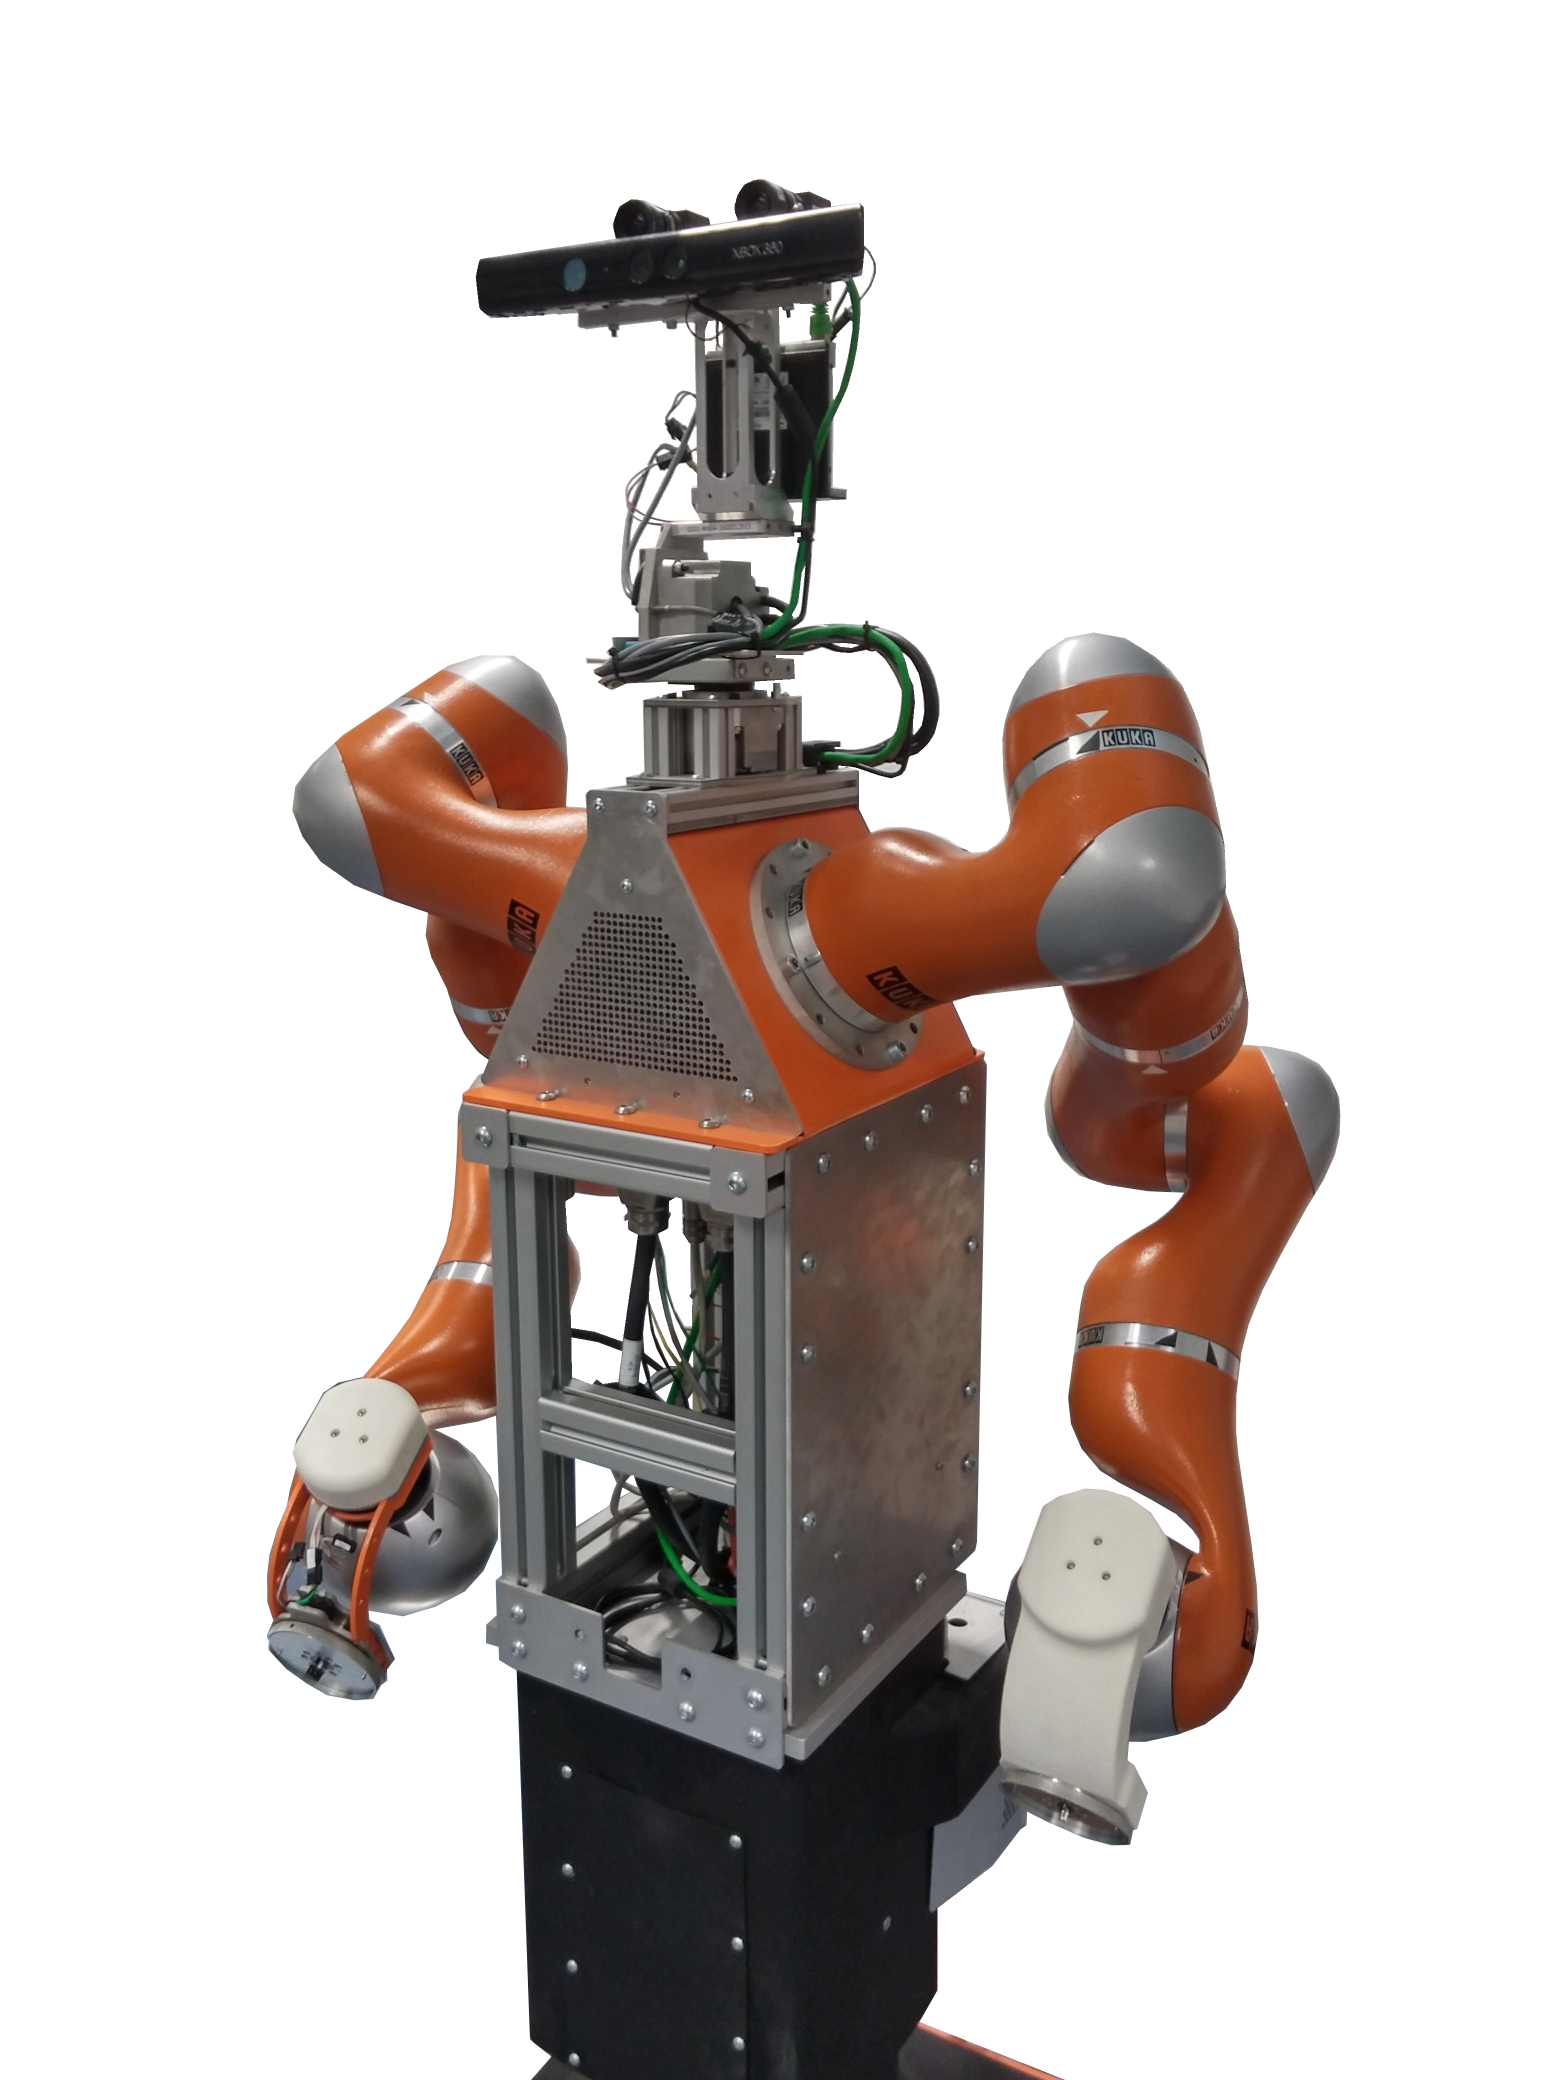
\includegraphics[width=0.5\textwidth]{graphics/velma.png}
	\caption{Robot manipulacyjny Velma.}
	\label{fig:velma}
	\end{figure} 

	Platforma jest niesymetrycznie podzielona na dwie części, przednią i tylną, w sposób pokazany na rysunku \ref{fig:base_ortho}.
	Przegub o jednym stopniu swobody (tzw. zawias) jest jedynym łącznikiem pomiędzy tymi dwoma fragmentami.
	Zadaniem tego przegubu jest zmniejszanie wpływu nierówności podłoża na ruch bazy, aby każde koło zachowało stały kontakt z podłożem.
	Bez tego przegubu, ruch po nierównym terenie uniemożliwiałby sprawne sterowanie platformą na skutek nieprzewidywalnych zaników tarcia kół o podłoże, powodując nieplanowane skręty.
	Takie zaniki tarcia kół są niewykrywalne w bezpośredni sposób, jak to zostało opisane w \cite{boringbot}.

	Platforma ma kształt prostokąta, jest 4 cm różnicy między szerokością, a długością robota.
	Koła są ustawione w wierzchołkach tego prostokąta.
	Szerokość jest większa, co można zobaczyć porównując widok z prawej strony, z widokiem z tyłu, rysunek \ref{fig:base_ortho}.
	Dokładne wymiary są podane na rysunku \ref{fig:base_dims} i tabeli \ref{tab:dims}.

	Platforma może w trakcie hamowania poruszać się innym kierunku, niż tuż przed zatrzymaniem.
	Jest to spowodowane tym, że konstrukcja rolek powoduje poślizg platformy w kierunku rolki mającej aktualnie kontakt z podłożem, a ten kierunek zależy od aktualnej
	orientacji bazy, nie od kierunku w jakim się porusza.
	Należy także wziąć tutaj pod uwagę inne cechy budowy kół, jak nierówne tarcie poszczególnych rolek o powierzchnię, 
	które może obrócić ten kierunek hamowania w nieprzewidywalny sposób \cite{braking}.

	\begin{figure}[H]
	\centering
	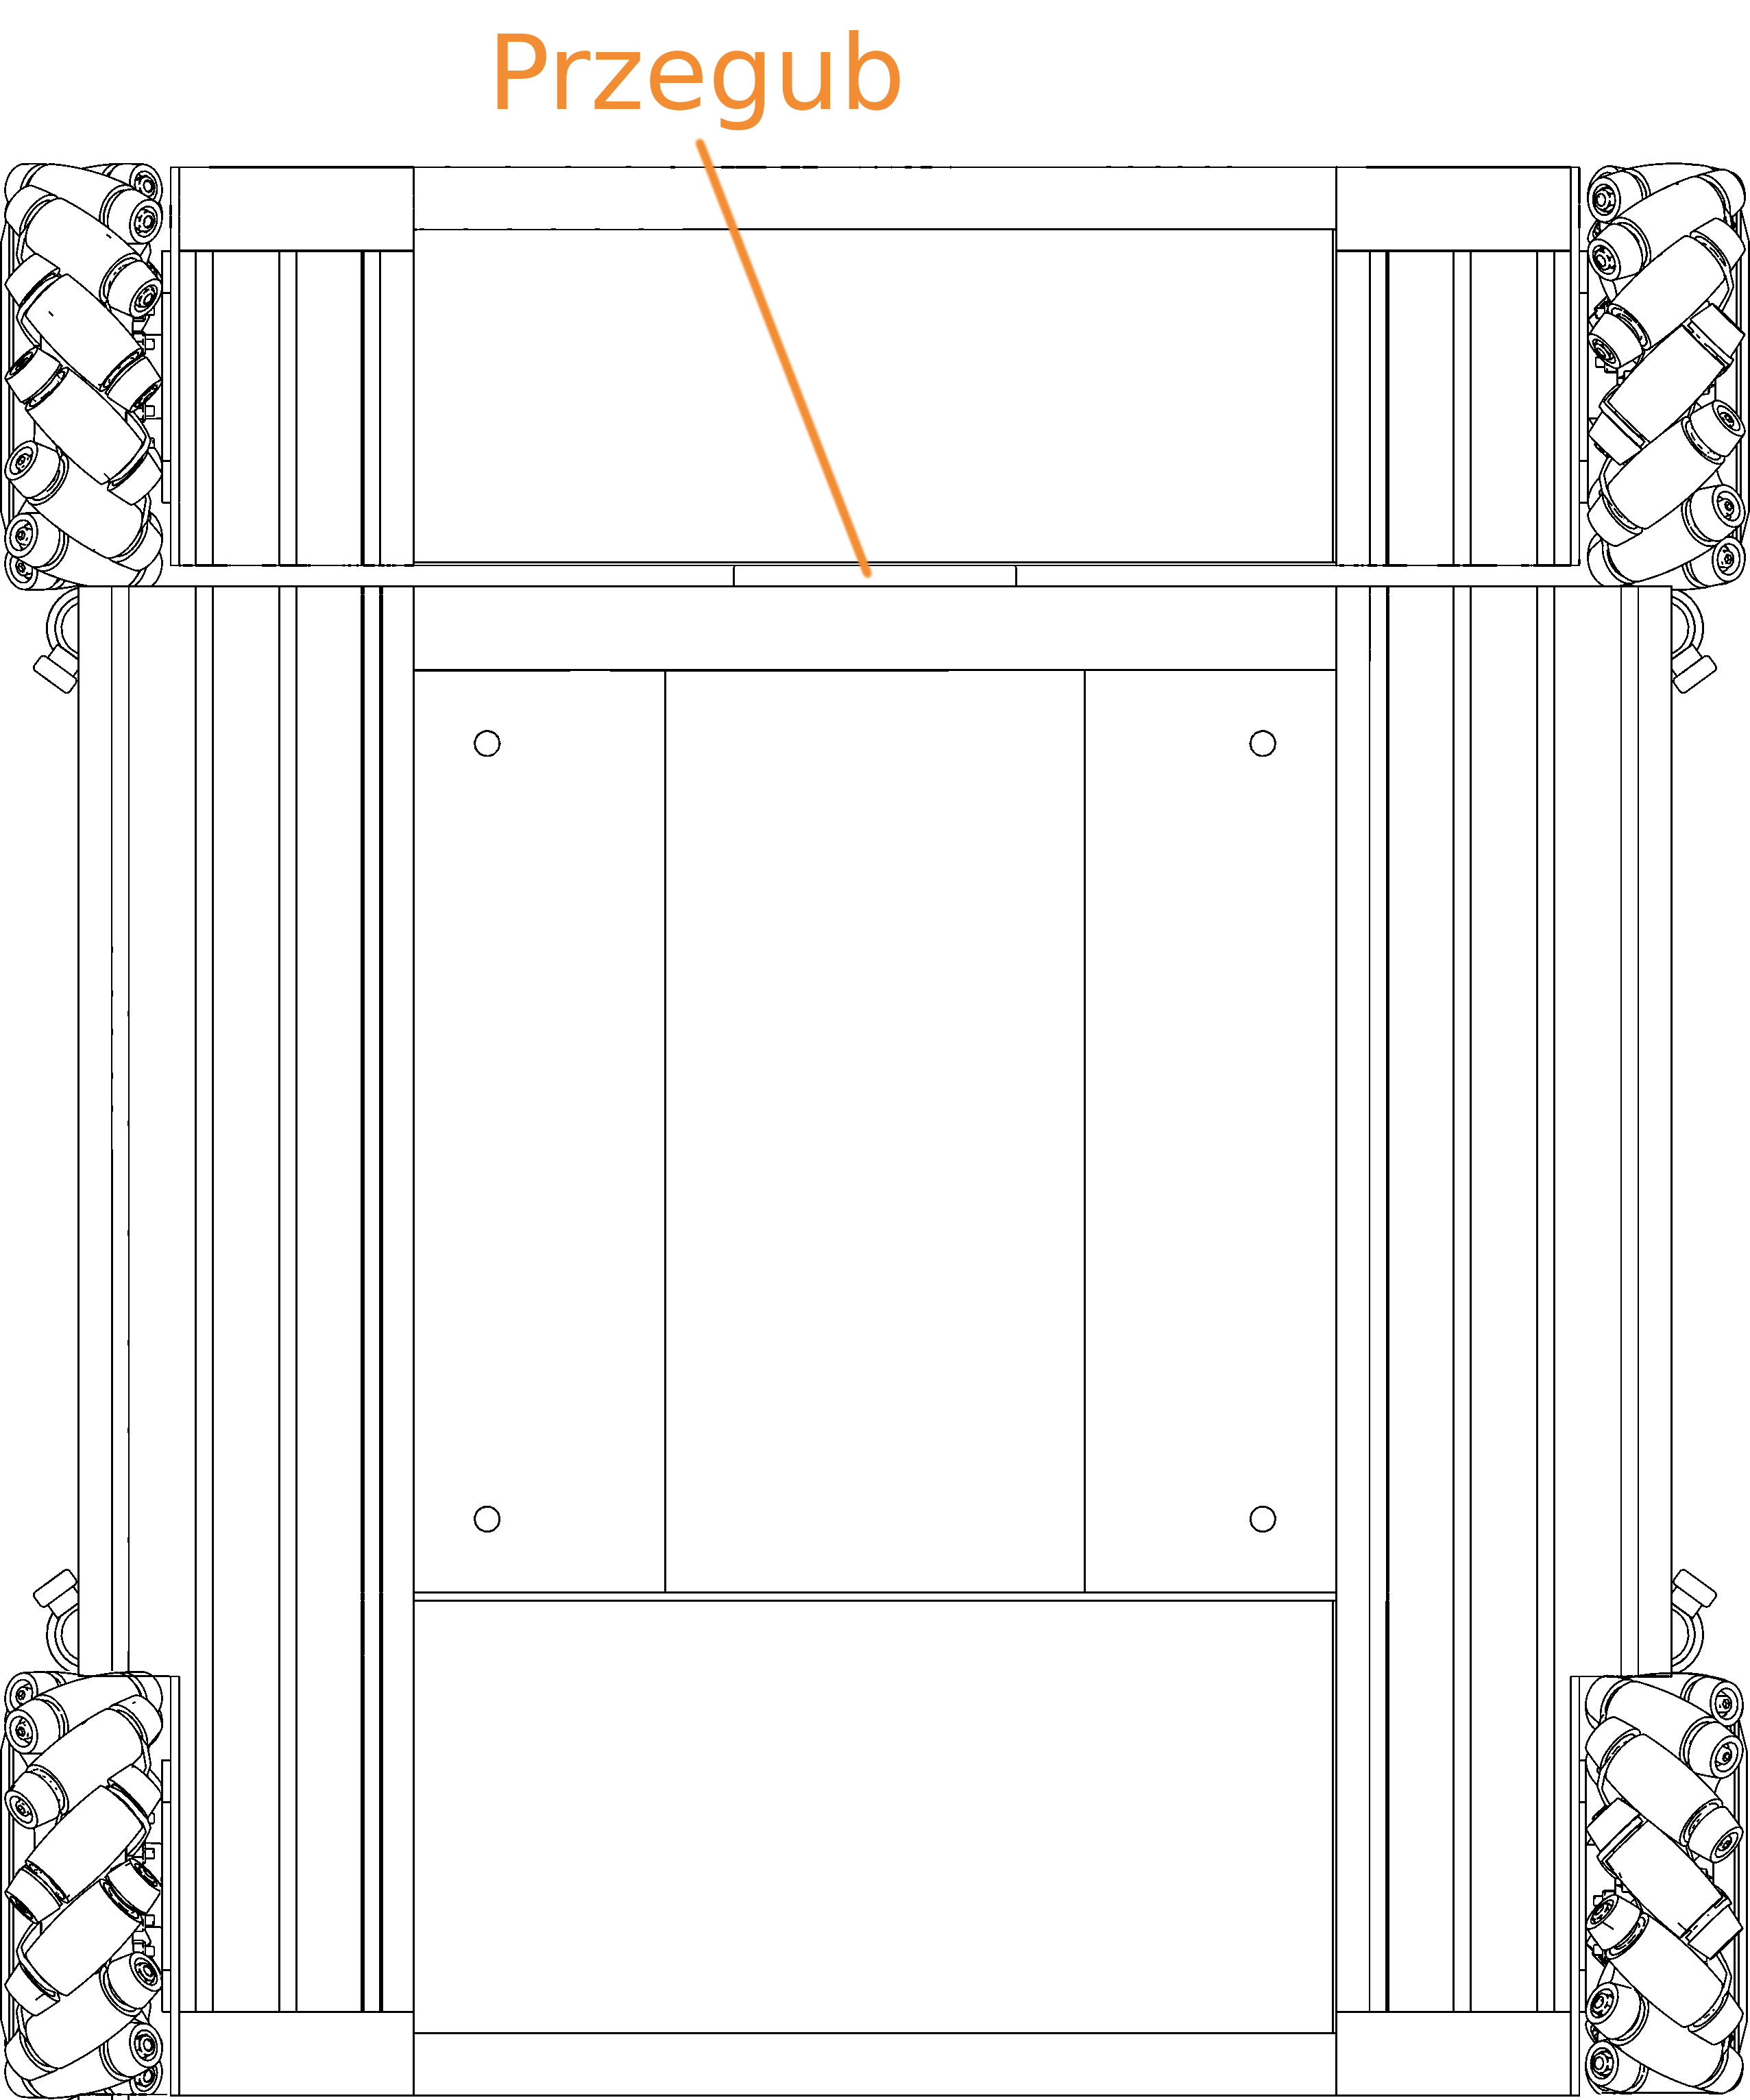
\includegraphics[width=0.5\textwidth]{graphics/base_top.png}
	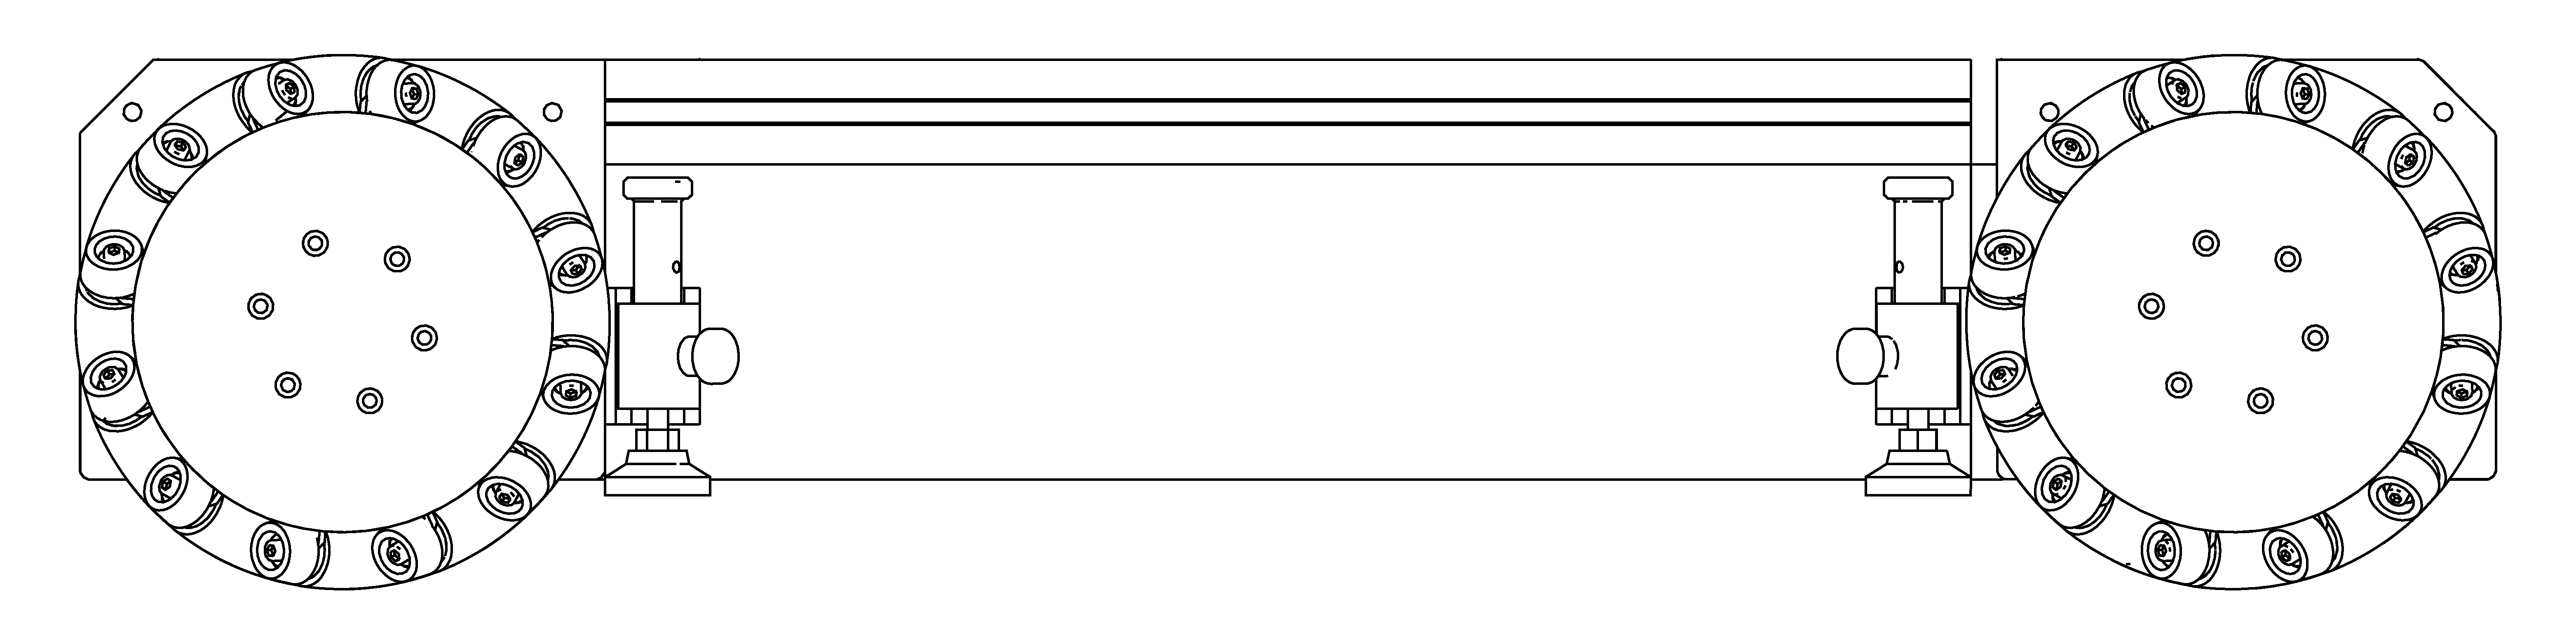
\includegraphics[width=0.62\textwidth]{graphics/base_side.pdf}
	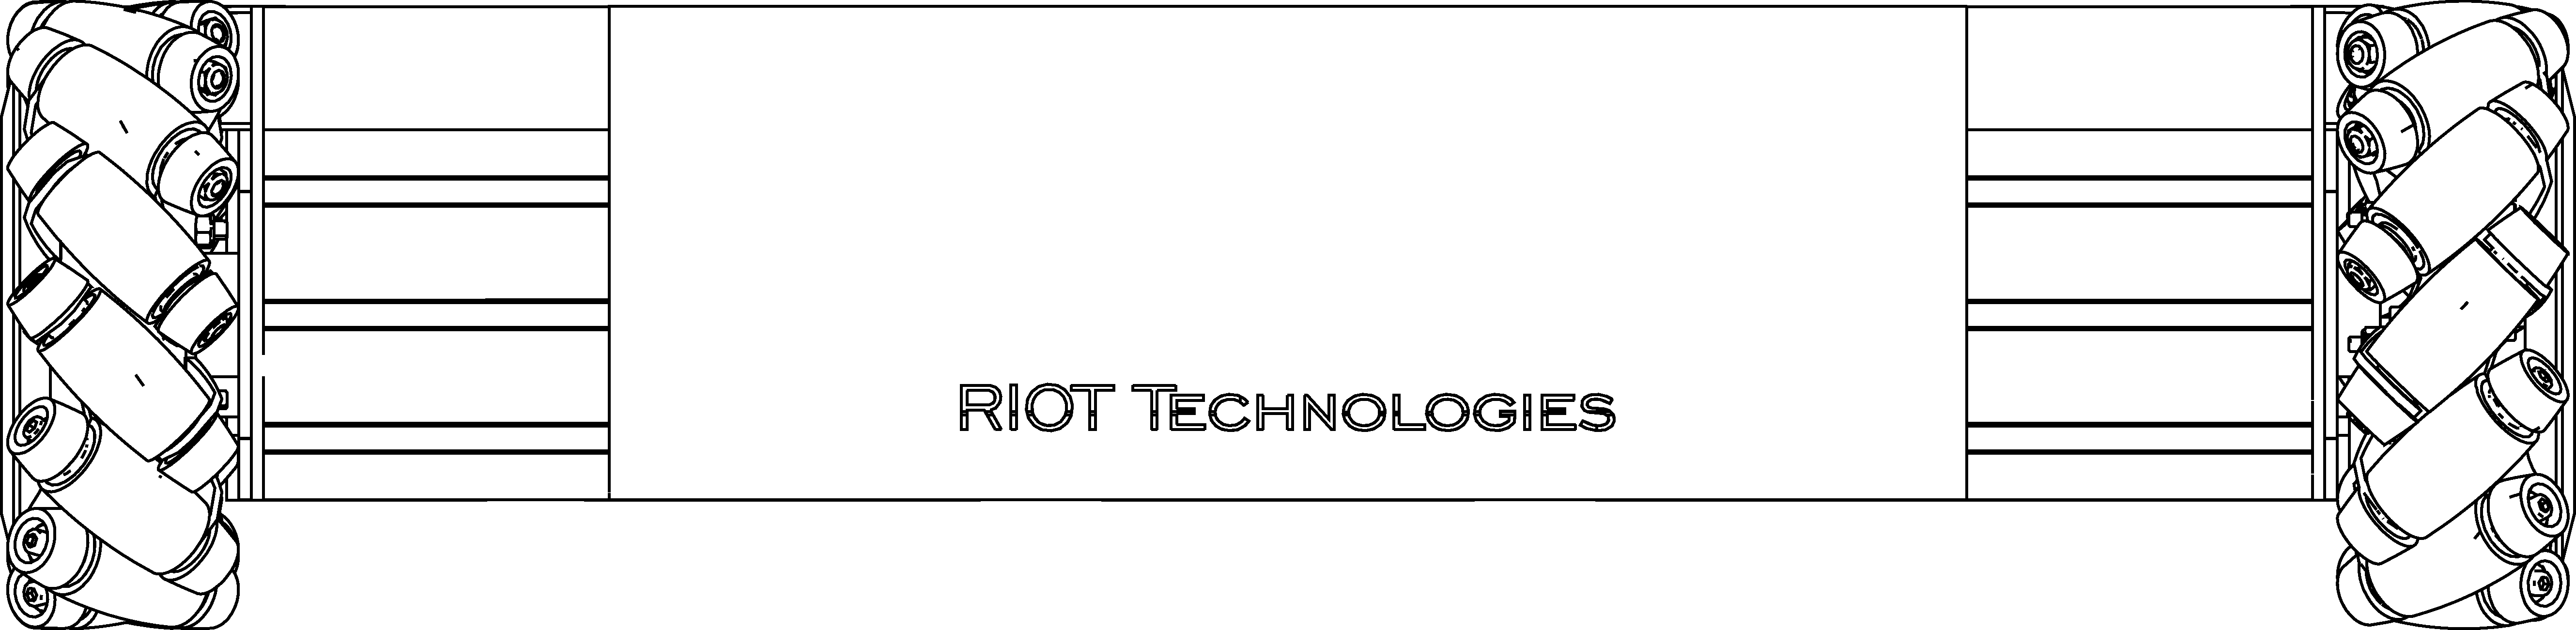
\includegraphics[width=0.62\textwidth]{graphics/base_front.pdf}
	\caption{Platforma mobilna. Widoki od góry, od prawej strony i od tyłu. Przegub obrotowy łączy dwie części.}
	\label{fig:base_ortho}
	\end{figure} 

	Platforma ma 3 stopnie swobody. 
	\begin{itemize}
		\item Przesunięcie wzdłuż osi X.
		\item Przesunięcie wzdłuż osi Y.
		\item Obrót wokół osi prostopadłej do podłoża.
	\end{itemize}
	
	Kierunek osi X i Y jest zgodny z ustalonymi dla programów sterujących platformą.
	
	\begin{figure}[H]
		\centering
		\includegraphics[width=0.8\textwidth]{graphics/base_dims.pdf}
		\caption{Wielkości używane we wzorach.}
		\label{fig:base_dims}
	\end{figure} 

	\begin{table}
		\centering
		\begin{tabular}{c c l}
		Oznaczenie & Wartość & Opis \\
		\hline
		$r$ & 0,1 m & Promień koła. \\
		$a$ & 0,76 m & Rozstaw kół na tej samej osi. \\
		$b$ & 0,72 m & Rozstaw osi. \\
		$\omega_i$ & & Prędkość kątowa $i$-tego koła. \\
		$v_x$ & & Składowa prędkości liniowej wzdłuż osi X. \\
		$v_y$ & & Składowa prędkości liniowej wzdłuż osi Y. \\
		$\omega_z$ & & Prędkość kątowa wokół osi Z, wektor skierowany w górę. \\
		\end{tabular}
		\caption{Parametry i zmienne modelu.}
		\label{tab:dims}
	\end{table}

\section{Koła szwedzkie}
	Koła szwedzkie, zwane także kołami Mecanum, to specjalne koła z dodatkowymi rolkami na obwodzie, ustawionymi pod kątem $45^\circ$ do osi koła.
	Rolki są pasywne i obracają się niezależnie od siebie. Każde koło ma 12 takich rolek, patrz rysunek \ref{fig:wheel}.
	W platformie ich osie ustawione są w ten sposób, że osie najwyższych, lub najniższych, rolek dwóch kół z tej samej strony robota przecinają się pod kątem prostym.
	Innymi słowy, robot ma identycznie ustawione koła na przeciwległych wierzchołkach, i razem ustawione są w kształt litery \emph{X}, patrząc na nie z góry.
	Należy pamiętać, iż oś aktualnie dolnej rolki jest prostopadła do osi górnej rolki.

	Istnieje również odwrotna odmiana ustawienia kół, w której rolki tworzą literę \emph{O}, 
	czyli oś przednia jest zamieniona z tylną, lub jakby cała platforma była odwrócona.
	Ten drugi sposób także pozwala na ruch wielokierunkowy, ale nie jest tak często stosowany \cite{paletobot}.

	\begin{figure}[H]
	\centering
	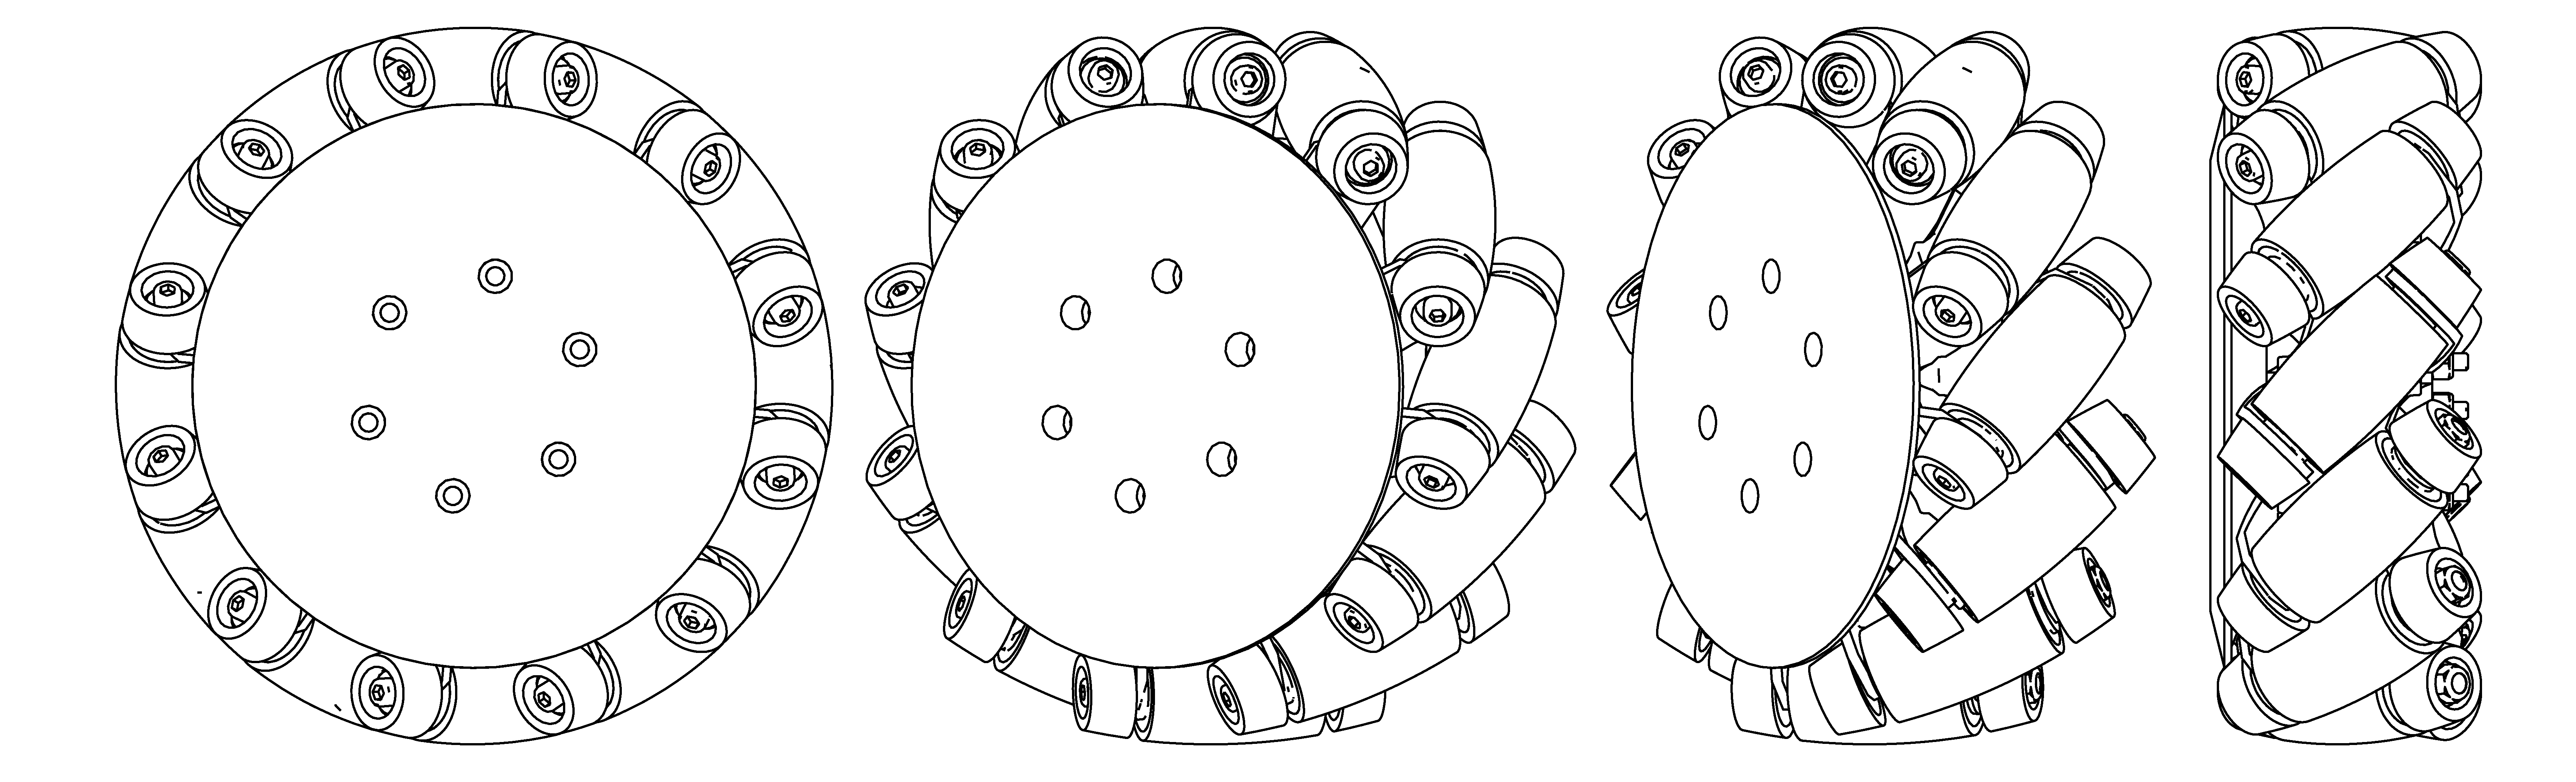
\includegraphics[width=\textwidth]{graphics/wheel.pdf}
	\caption{Widok 12 rolkowego koła szwedzkiego platformy wielokierunkowej.}
	\label{fig:wheel}
	\end{figure} 

	Każde koło ma 3 stopnie swobody \cite{kinematic_modeling}, tak samo jak cała platforma.
	\begin{itemize}
		\item Obrót koła w osi prostopadłej do płaszczyzny koła i przechodzącej przez jego środek.
		\item Rotacje pojedynczych rolek.
		\item Poślizg rolki w miejscu styku rolki z podłożem.
	\end{itemize}

	Na podstawie rysunku \ref{fig:wheel} można zauważyć, że krzywizna rolki jest tak ustawiona, aby punkt kontaktu rolki z podłożem w czasie obrotu koła płynnie przechodził na następną rolkę.
	Celem jest utrzymanie równej odległości osi obrotu koła od płaszczyzny podłoża.
	Nie powinno być efektu przeskoku z jednej rolki na drugą, gdyż to wprowadza nierówne tarcie, losowe poślizgi i nadmierne zużycie elementów wykonawczych.
	Kształt pojedynczej rolki jest wycinkiem paraboloidy, wzory opisujące kształt rolki są złożone.
	Zazwyczaj przybliża się taką rolkę wycinkiem torusa, w celu uproszczenia produkcji \cite{rollers}.

	Istnieją także koła o innej konstrukcji, złożone z wielu małych rolek, tak aby w każdym momencie więcej jak jedna rolka dotykała podłoża.
	Można także złożyć kilka powyższych kół obok siebie w jedno koło.
	Przydatne jest to dla robotów transportujących duże masy, gdyż zmniejsza to obciążenie pojedynczych rolek.
	Niestety, taka konstrukcja jest chroniona aktywnym patentem, więc pojedyncze koło, na które patent już wygasł, jest jedynym powszechnie używanym \cite{paletobot}.

	Podstawowym problemem konstrukcji koła jest nie tylko skomplikowana budowa, ale także ślizganie się rolek po powierzchni.
	Odległość osi obrotu koła od płaszczyzny podłoża nieznacznie zmienia się przy przenoszeniu ciężaru z rolki na rolkę, co przy dużych prędkościach powoduje drgania i jeszcze większe błędy szacowania pozycji

	\subsection{Ruch platformy na kołach}
		W zwykłym kole, dzięki tarciu, moment obrotu przekształcany jest na przyspieszenie w kierunku równoległym do podłoża i płaszczyzny koła.
		Dodatkowo wektory tarcia są równe we wszystkich kierunkach. To znaczy, koło będzie stawiało identyczny opór, niezależnie czy siła
		zostanie przyłożona wzdłuż osi obrotu koła, czy równolegle do płaszczyzny podłoża i płaszczyzny rolki.
		
		Specjalne koło Mecanum wywołuje tarcie kierunku obróconym o 45° w stosunku do osi obrotu koła, zależnie od typu koła (prawoskrętne lub lewoskrętne). 
		To oznacza, że przy nadaniu momentu siły $I$, wektor tarcia koła o powierzchnię $T$ będzie obrócony w stosunku do osi obrotu koła o 45°.
		Z kolei tarcie nada kołu siłę $F$ o przeciwnym zwrocie do wektora tarcia.
		Tarcie w kierunku $f_0$, prostopadłym do $F$, czyli zgodnie z obrotem najniżej położonej rolki, jest w idealnym przypadku zerowe.
		Z kolei wypadkowa siła od wszystkich kół nadaje platformie przyspieszenie i prędkość w odpowiednim kierunku.

		\begin{figure}[H]
		\centering
		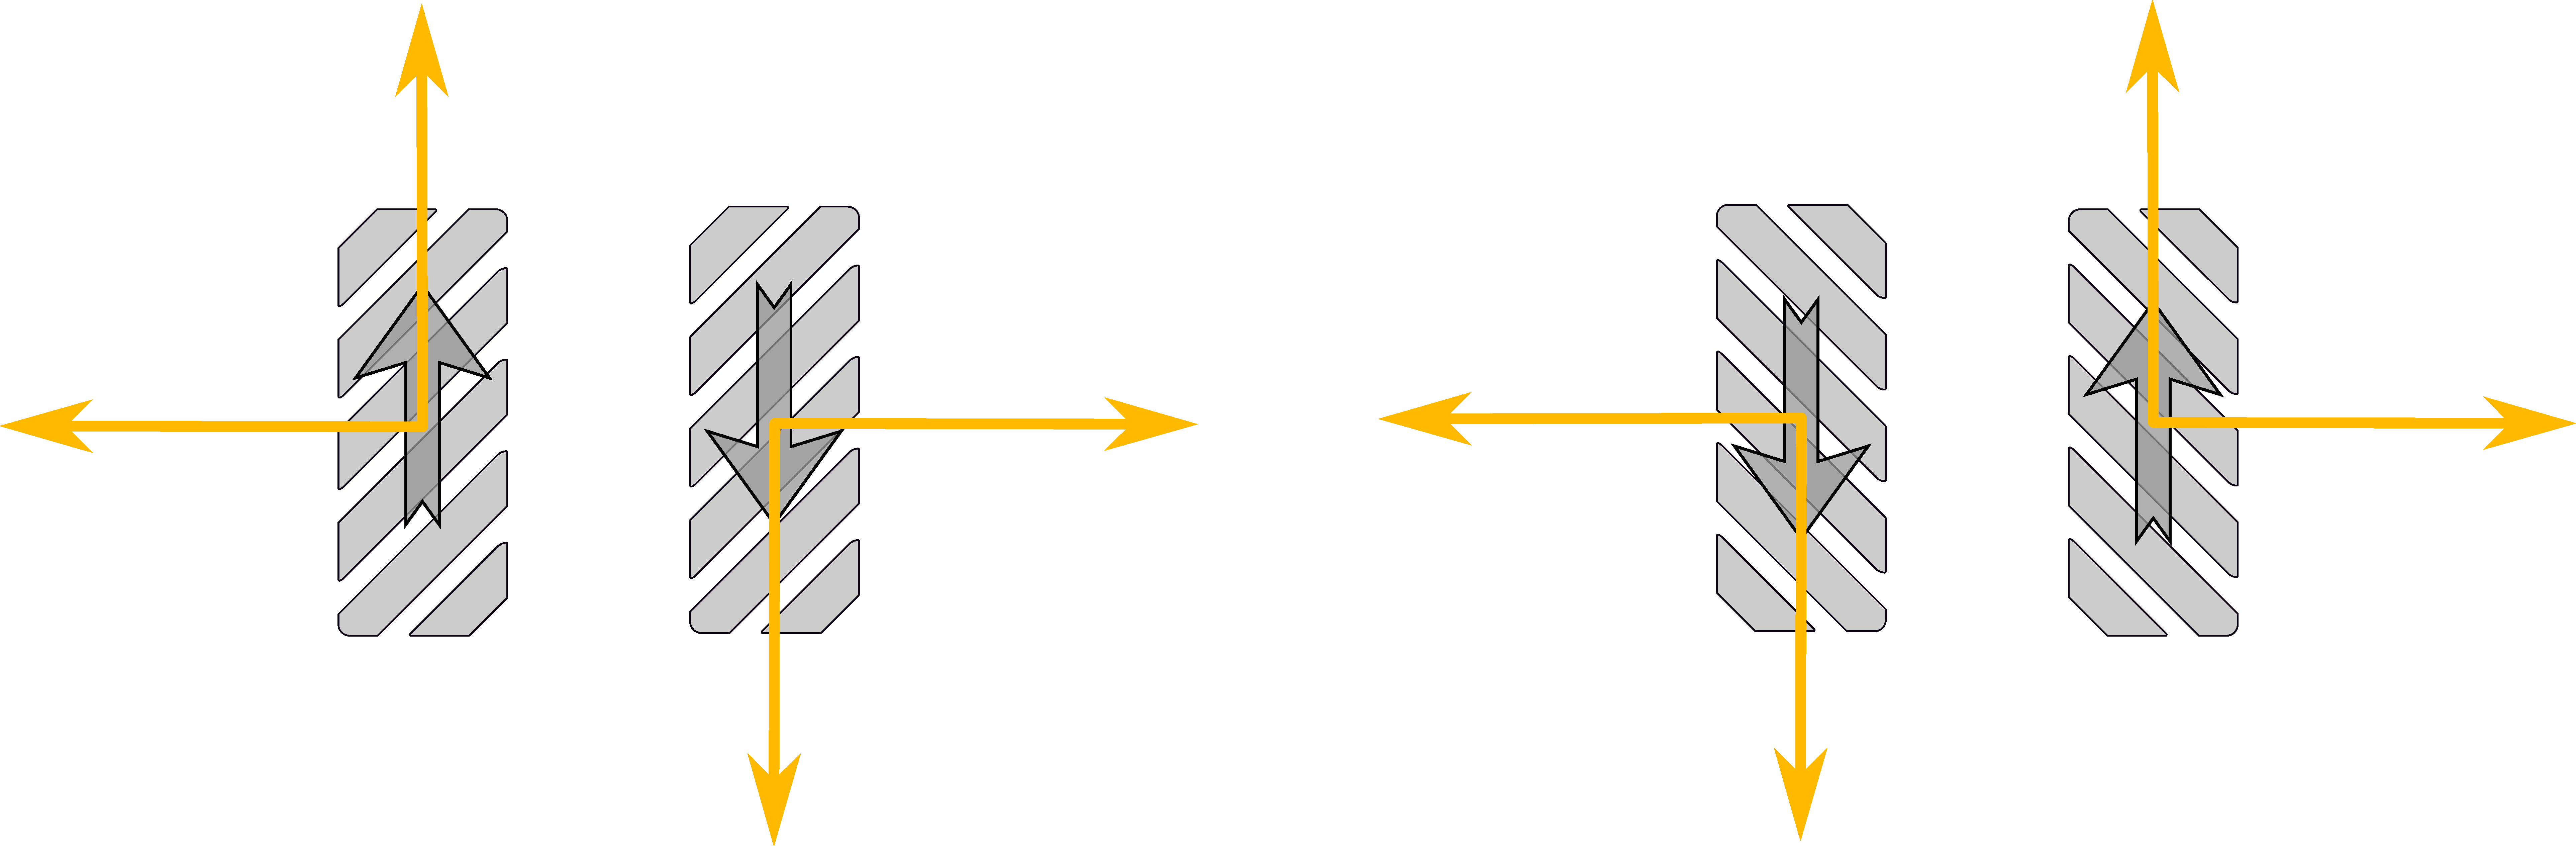
\includegraphics[width=\textwidth]{graphics/vectors.pdf}
		\caption{Wektory momentu siły i siły koła Mechanum, widzianego z góry.}
		\label{fig:wheel_vectors}
		\end{figure} 

		Ustawiając te koła w odpowiedni, pokazany na rysunku \ref{fig:base_dims}, sposób, można wywołać odpowiednie znoszenie się składowych sił,
		a w efekcie pozwolić robotowi na poruszanie się w kierunkach nieosiągalnych dla pojazdów o standardowych kołach.
		Warto nałożyć te wektory na wcześniejszy rysunek \ref{fig:mecanum_dirs}, aby dokładniej zobaczyć, 
		dlaczego koła nadają platformie daną prędkość wypadkową przy odpowiednim obrocie kół.

		\begin{figure}[H]
		\centering
		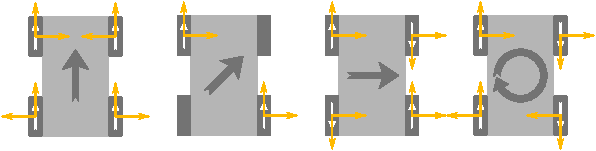
\includegraphics[width=\textwidth]{graphics/mecanum_dirs_vect.pdf}
		\caption{Ruchy platformy widzianej z góry, z nałożonymi składowymi wektorów sił.}
		\label{fig:mecanum_dirs_vect}
		\end{figure} 

		Warto rozpatrzyć każdy przypadek. Platforma posiada jedną płaszczyznę symetrii, ze względu na asymetryczny przegub.
		\begin{enumerate}
			\item Składowe wektorów sił o kierunku prostopadłym do pionowej płaszczyzny symetrii urządzenia znoszą się, ponieważ mają przeciwne zwroty na lewej i prawej parze kół.
			Pozostają jedynie składowe równoległe do płaszczyzny symetrii, które powodują prostoliniowy ruch naprzód.
			\item Dwa koła nie obracają się. Nie jest to ruch pasywny, gdyż taki wprowadzałby nieprzewidywane poślizgi, a aktywne hamowanie.
			Wektory się nie znoszą i platforma wykonuje ruch pod kątem 45° do płaszczyzny symetrii. Ruch odbywa się równolegle do kierunku $f_0$ zatrzymanych kół,
			zatem nie stawiają one w tym momencie oporu.
			\item Ruch podobny jest do przypadku 1. Tutaj również wektory znoszą się parami, jednak tym razem na przednich parach i tylnych. 
			Pozostają składowe prostopadłe do płaszczyzny symetrii, które nadają platformie przyspieszenie w bok.
			\item Prędkość kątowa powstaje, gdy wypadkowa kół po jednej stronie platformy znosi się z wypadkową po drugiej stronie.
		\end{enumerate}

		Warto nadmienić, że gdy wypadkowy wektor prędkości koła jest prostopadły do osi koła, to jest gdy
		koło porusza się zgodnie z kierunkiem obrotu, w idealnym przypadku rolki nie obracają się.
		Inaczej mówiąc, rolka będzie się obracać tym mocniej, im bardziej ruch koła wymuszany jest równolegle do osi koła, 
		czy to na skutek znoszenia się wektorów, czy oporu przeszkody.
		
		Przykładowo, przy ruchu naprzód, rolki koła się nie obracają, lecz przy ruchu w bok biorą aktywny udział.
		Ma to wpływ na zużywanie się tych elementów, nie tylko z punktu widzenia ilości obrotów danej rolki na pokonanym dystansie, 
		ale także sposobu w jaki wymuszany jest jej ruch.
		Rolki robota przy jeździe zawsze obracają się szarpanym ruchem w obie strony, ze względu na poślizgi od innych kół, 
		niejednostajne tarcie piast wszystkich rolek, czy różnice terenu. 
		Zatem przejazd przykładowego odcinka, przy platformie ustawionej przodem do kierunku jazdy, lub bokiem, będzie w różnym stopniu i w różny sposób zużywał elementy wykonawcze robota.
		To, jak dokładnie zużywają się przeguby i jaki styl jazdy opłaca się zastosować, aby zminimalizować uszkodzenia elementów jest dużą, odrębną dziedziną nauki.
		Odpowiednio skomplikowany algorytm sterowania może brać pod uwagę tą mechanikę kół.

\section{Enkodery}
	Każde koło posiada wbudowany w silnik enkoder. To urządzenie wykrywa aktualny ruch koła i zwraca jego aktualną prędkość i rotację.
	Korzystając z modelu kinematyki, można obliczyć z tych danych wypadkową prędkość robota, a następnie, za pomocą całkowania, wyznaczyć aktualną
	pozycję w stosunku do punktu startowego.
	
	W opisywanym robocie, silniki kół mają na tyle dużą moc, że wartość prędkości, wykrytej przez enkodery, bardzo niewiele odstaje od prędkości zadanej.
	Oznacza to, że teoretycznie, można nadawać kołom bardzo duże momenty sił, a koło rzeczywiście wykona zadaną akcję.
	Jednakże eksperymenty pokazały, że zasilacz robota może nie móc pracować przy takim poborze prądu i awaryjnie się odłączyć, co jest głównym powodem dla którego 
	należy ograniczać nadawanie zbyt dużych przyspieszeń platformie.

	Poślizg kół powoduje jednak, że odometria, bazująca na danych generowanych przez czujniki enkoderów, obarczona jest błędami losowymi i nie może być 
	użyta jako jedyna metoda wyznaczania pozycji względnej w trakcie jazdy robota \cite{heavy}. Zatem dodano do urządzenia także inne czujniki.
	
\section{Skaner laserowy}
	\label{sec:lidar}
	Dodatkowym czujnikiem, używanym przy wyznaczaniu pozycji platformy, jest skaner laserowy.
	Platforma wyposażona jest w dwa, dwuwymiarowe czujniki typu LiDAR firmy SICK.
	LiDAR to połączenie wyrazów \emph{light} i \emph{radar}, chociaż skrót może być rozwinięty w różne słowa.

	\begin{figure}[h]
	\centering
	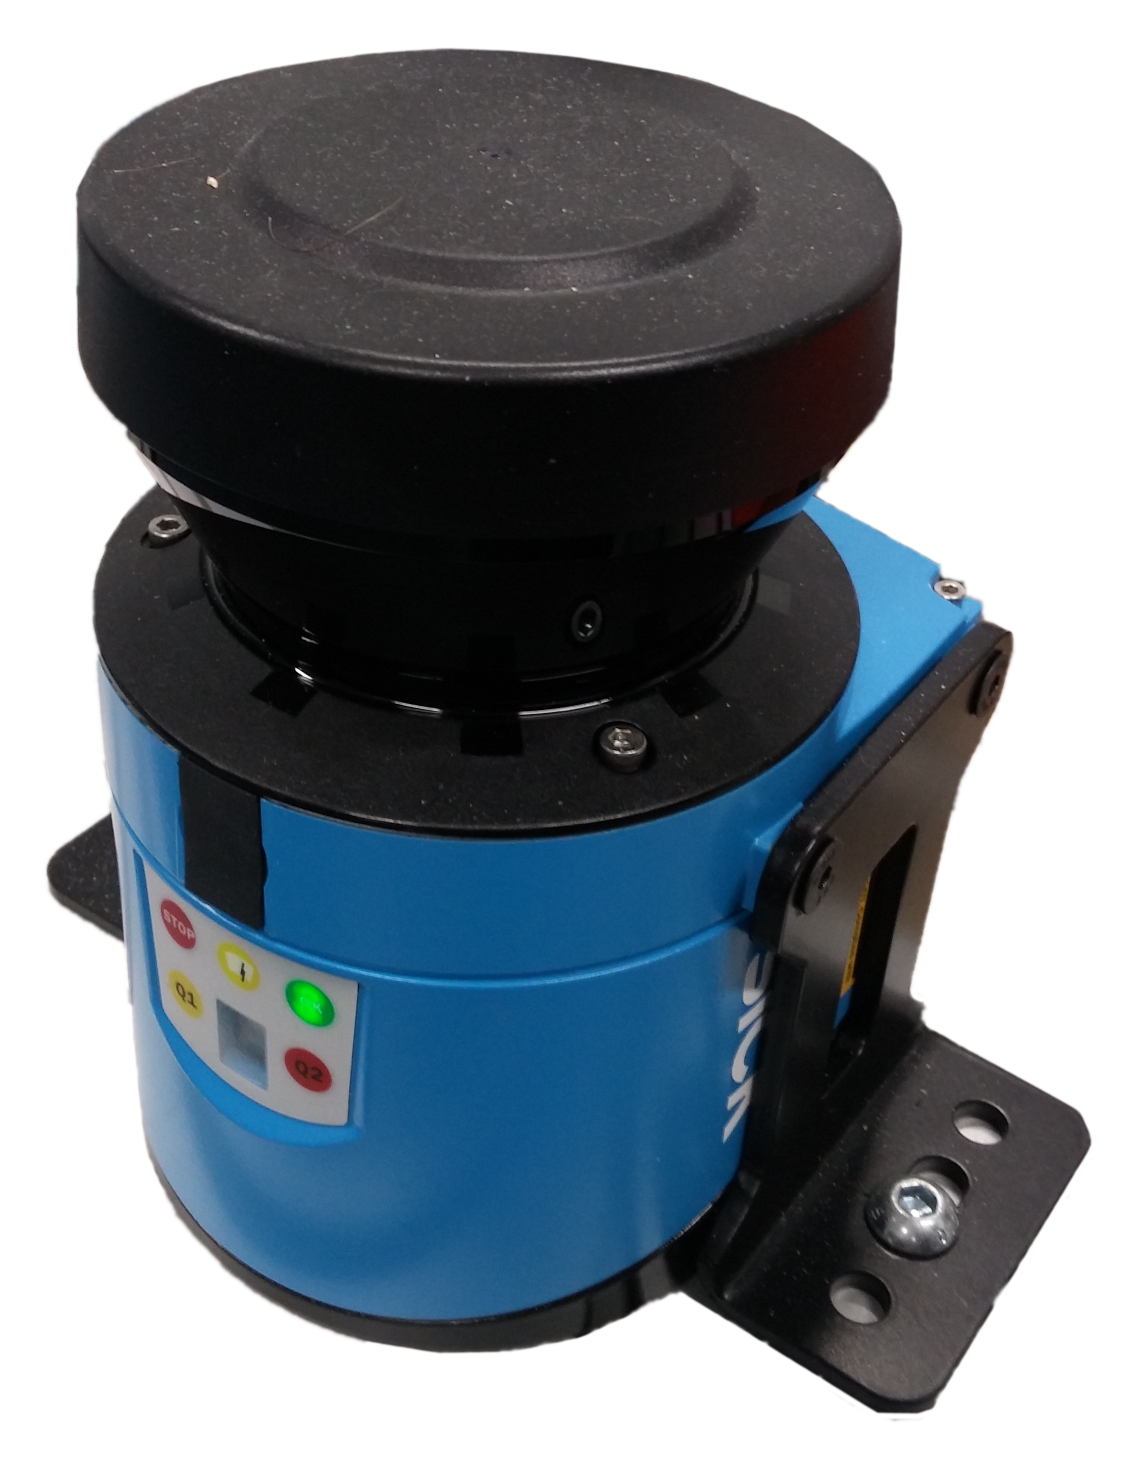
\includegraphics[width=0.5\textwidth]{graphics/sensor.png}
	\caption{Skaner laserowy SICK LMS100-10000.}
	\label{fig:sensor}
	\end{figure} 

	\subsection{Zasada działania}
		Wszystkie skanery tego typu mają bardzo podobną zasadę działania.
		W środku urządzenia znajduje się obrotowe lusterko, zwrócone pod kątem 45° do osi obrotu.
		Równolegle do osi jego obrotu znajduje się laser, który emituje pulsacyjną wiązkę podczerwonego promienia co pewien okres czasu.
		Emitowanie stałego promienia może być niebezpieczne dla wzroku obsługujących go ludzi.
		Aktualna pozycja lusterka jest wykrywana przez enkoder.
		Obok lasera jest czujnik, który bada wysłane przez laser, odbite od lusterka, obiektu i ponownie lusterka, światło.

		Na koniec, algorytm we wbudowanym mikrokontrolerze ustala kąt i odległość czujnika od wykrytego obiektu.
		Odpowiada także za usunięcie szumu i ewentualnych odbić promienia.
		Komunikacja z urządzeniem może odbywać się za pomocą różnych interfejsów sieciowych, zazwyczaj w architekturze typu master-slave.
		W przypadku tej platformy jest to Ethernet.
		
		Skośna szyba, będąca wycinkiem powierzchni stożka, zabezpiecza wnętrze przed zanieczyszczeniami, jej kształt niweluje ewentualne odbicia lasera, emitowanego poziomo ze środka.
		W niektórych czujnikach montuje się także szereg dodatkowych diod podczerwieni na obrębie szyby, skierowanych w górę, lub w dół, oraz czujniki/reflektory z drugiej strony.
		Pozwala to na wykrycie stopnia zanieczyszczenia szyby, aby powiadomić użytkownika o potrzebie wyczyszczenia urządzenia.

	\subsection{Komunikacja}
		Wysyłając do czujnika odpowiedni ciąg bajtów, można ustawić jego tryb działania, odpytać o zebrane dane, czy wykryć konfigurację i stan.

		W przypadku tej platformy, komunikacja odbywa się poprzez interfejsy EtherCAT i Ethernet.
		EtherCAT to sposób komunikacji urządzeń po kablu Ethernetowym, w trybie \emph{master}-\emph{slave}, przy zachowaniu sztywnych ram czasowych. 
		\emph{Master} wysyła pakiet do podłączonych szeregowo urządzeń \emph{slave}, które przekazują go przez siebie i w razie potrzeby modyfikują dane w locie.
		
		Program odbierający dane od czujnika komunikuje się bezpośrednio z urządzeniem, które zwraca pakiety zawierające pomiary z ostatniego obrotu czujnika, oraz dodatkowe dane 
		opisujące sam pomiar, takie jak czas, początkowy kąt pomiaru, czy tryb pracy.
		Dokładne pola w pakiecie i cechy czujnika dostępne są na stronie producenta \cite{sick_website}.

		Urządzenie wspiera uwierzytelnianie przez hasło, wgrywanie nowego oprogramowania,
		ustawienia czasu, oraz zmianę różnych parametrów działania.

	\subsection{Podstawowe cechy}
		Czujnik składa się z dwóch części, głównego trzonu, oraz nakładki.
		Połączenie tych elementów powoduje, że jego zakres pomiaru posiada martwy kąt.
		Przedstawia to dobrze grafika producenta \ref{fig:lidar}.
		\begin{figure}[h]
		\centering
		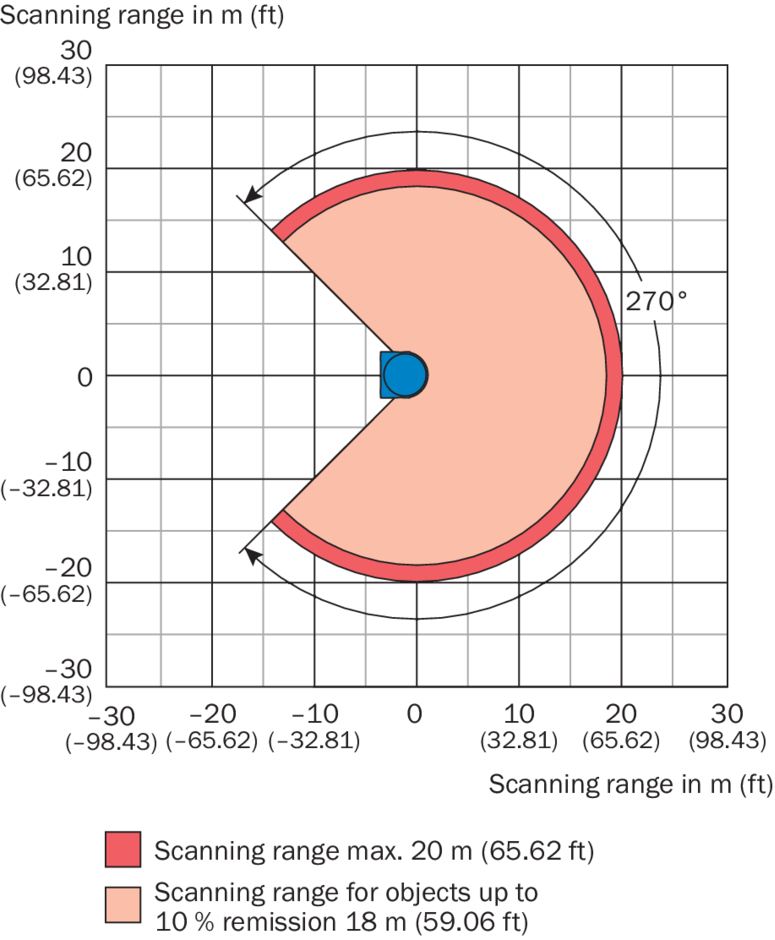
\includegraphics[width=0.6\textwidth]{graphics/sick.png}
		\caption{Wykres producenta dotyczący zasięgu czujnika \cite{sick_website}.}
		\label{fig:lidar}
		\end{figure} 
		
		\begin{table}
		\centering
		\begin{tabular}{l r}
		Cecha & Wartość \\
		\hline
		Kąt pracy & 270\textdegree \\
		Długość fali światła lasera & 905 nm (podczerwień) \\
		Częstotliwości skanowania & 25 Hz / 50 Hz \\
		Maksymalna odległość obiektu & $\approx$ 20 m \\
		Rozdzielczość kątowa & $0,25 \degree$ / $0,5 \degree $ \\
		Systematyczny błąd pomiarowy & $\pm 0,03$ m \\
		Przypadkowy błąd pomiaru odległości & $0,012$ m \\
		\end{tabular}
		\caption{Podstawowe cechy czujnika laserowego.}
		\label{tab:lidar}
		\end{table}
		Na podstawie tych danych można obliczyć, że w jednym przebiegu po całym zakresie kątowym urządzenia, 
		emitowane jest około 1080, lub 540 impulsów (w zależności od trybu działania).
		Taka liczba promieni wymagana jest w symulacji, aby wiernie odwzorować urządzenie.

\section{Jednostka inercyjna}
	Ten czujnik to małe urządzenie, posiadające zazwyczaj zestaw wewnętrznych czujników, przydatnych przy określaniu prędkości, rotacji i przyspieszeń modułu.
	Dodatkowo, wiele zestawów tego typu posiada także czujniki pola magnetycznego, położenia, lub nawet termometry.
	
	Czujnik użyty w platformie to ADIS16460AMLZ, firmy Analog Devices. Szczegółowa dokumentacja jest dostępna na stronie sprzedawcy \cite{adis_website}.
	
	Urządzenie ma kształt małej kostki i komunikuje się za pomocą złącza SPI, a co za tym idzie, wymaga zewnętrznego mikrokontrolera, aby móc wysyłać wygenerowane dane
	do sieci do innych urządzeń.
	
	Czujnik jest wyposażony w:
	\begin{itemize}
		\item Trzyosiowy żyroskop.
		\item Trzyosiowy akcelerometr.
		\item Czujnik temperatury.
		\item Sprzętowe wspomaganie korekcji błędów i kalibracji.
	\end{itemize}
	
	Błędy pomiarowe akcelerometra są bardzo duże, w stosunku do błędów pomiarowych żyroskopu i skanera laserowego. 
	Aby użyć tych danych w programie, należy zastosować na nich algorytmy usuwające szum i uśredniające wyniki.
	Rysując dane zebrane bezpośrednio z czujnika na wykresie, można jedynie z małą dokładnością określić kierunek przyspieszenia działającego na platformę, ale nie jego 
	wartość.
	
	W symulacji nie jest używana informacja o temperaturze otoczenia, zatem nie ma potrzeby jej symulować.
	
\section{Podłączenie urządzenia}
	Platforma podłączona jest do dedykowanego komputera, który pracuje z systemem operacyjnym Ubuntu i dodatkowymi modułami, które zapewniają 
	pracę w czasie rzeczywistym, aby urządzenie mogło poprawnie współpracować z robotem.
	
	Na tym systemie pracuje program, który przyjmuje komendy z innej sieci, odbierane z innego, biurowego komputera.
	Są tutaj także uruchomione algorytmy, obliczające pozycję platformy, bazując na odometrii.
	
\section{Sterowanie urządzeniami}
	Efektory robota wymagają podania odpowiedniego sterowania, a czujniki odpowiedniego odbiornika.
	\subsection{Sterownik silników}
		Program sterujący generuje abstrakcyjne dane, na przykład liczbę zmiennoprzecinkową, zapisaną binarnie.
		Przykładowy silnik fizyczny nie jest w stanie działać na podstawie takich danych, do pracy potrzebuje odpowiedniego napięcia na wejściu.
		Do tłumaczenia jednych danych na drugie, potrzebny jest sterownik niskopoziomowy.
		Najczęściej implementowany jest w formie mikrokontrolera, lub podobnego systemu wbudowanego.

		Jego zadanie to odczytanie danych, podanych przez program sterujący i na przykład generowanie na ich podstawie odpowiedniego przebiegu PWM, lub obsługa przetwornika cyfrowo-analogowego.
		Do innych zadań może należeć kontrola, czy żądana wartość nie uszkodzi urządzenia.
		Zazwyczaj sterownik może komunikować się z powrotem z resztą systemu, aby zgłaszać ewentualne awarie.

		Taki program i powiązany z nim układ elektroniczny są najczęściej dostarczone przez producenta robota i nieznane użytkownikowi.
		Dodatkowo, tworzy to kolejną warstwę abstrakcyjną dla sterownika głównego, który nie musi zważać na generowanie różnych danych dla różnych modeli tych samych efektorów.
		
	\subsection{Sterownik czujników}
		Implementowany podobnie do sterownika silników, ma za zadanie konwertować surowe i obarczone błędami dane z czujników na format zrozumiały dla programu sterującego.
		W tym miejscu usuwa się błędy grube, niweluje stałe na podstawie kalibracji, wygładza szum i interpretuje dane, aby pozyskać wymagane przez wyższe warstwy informacje.

		Przykładowo, czujnik zwraca jedynie ciąg pomiarów, ale to do tego programu należy połączenie pomiaru z informacją o emisji promienia, na ich podstawie obliczenie odległości od przedmiotu i porównanie z innymi pomiarami w celu usunięcia błędów grubych.
		Większość zaawansowanych receptorów posiada owe układy cyfrowe i programy wbudowane w urządzenie.
		Dostarczone są przez producenta tak samo, jak sterowniki efektorów.
		
		Aby zasymulować ten element, należy zbudować program generujący dane na podstawie aktualnego stanu maszyny do symulacji, w sposób w jaki działa czujnik w rzeczywistości.
		Na przykład, dla czujnika laserowego, silnik symulacji fizycznej emituje odpowiednią ilość promieni i oblicza ich punkty przecięcia się z wirtualnymi modelami.
		Renderowanie obrazu pozwala na symulację kamery.

		Ponieważ dane fizyczne nigdy nie są idealne, w celu przybliżenia wyjścia wirtualnego czujnika do oryginału, dodaje się szum o odpowiednim rozkładzie i błędy.

	\subsection{Program sterujący}
		W programie sterującym obliczane jest sterowanie, na podstawie dostarczonych odczytów z czujników.
		Zazwyczaj wykorzystuje się tutaj także zewnętrzne biblioteki, dostarczające zaawansowane algorytmy.
		Ich zadania mogą polegać na budowie wewnętrznej mapy, wyznaczaniu ścieżki, omijaniu przeszkód, odwrotnej kinematyce i tym podobnych.

		Taki program zwykle działa na mocniejszych układach logicznych, niż sterowniki, ze względu na duże zapotrzebowania na moc obliczeniową
		i niedeterministyczny czas obliczeń.
		Jeśli robot komunikuje się z użytkownikiem, to zachodzi to w tym module. 

		Programy sterujące mogą być implementowane w językach wysokopoziomowych, nawet skryptowych, gdyż wymagania czasowe nie są rygorystyczne.
		Co więcej, często się zdarza, że odpowiednie składowe programu bazują na różnych technologiach.

		Środowisko symulacyjne powinno zapewnić pełną abstrakcję komunikacji tego modułu.
		Oznacza to, że niezależnie, czy program steruje rzeczywistym robotem, czy symulacją wirtualną, zawsze powinien móc komunikować się i otrzymywać dane w tym samym formacie.
		W idealnym przypadku program nie powinien mieć możliwości stwierdzić, czy steruje symulacją, czy fizycznym urządzeniem.
		
